% English manuscript. Compile with pdflatex -jobname=articlee_final until references stabilize (usually three passes).
% Compatibility for the unchanged November 2016 SIAM class on modern LaTeX.
% The class replaces \refstepcounter with a pre-hyperref implementation that
% does not set \@currentcounter; modern cleveref requires that information.
% Restore the kernel implementation before hyperref and cleveref wrap it.
% Load this small shim BEFORE \documentclass. No journal formatting is changed.
\let\ELAKernelRefstepcounter\refstepcounter
\AddToHook{package/hyperref/before}{\let\refstepcounter\ELAKernelRefstepcounter}

\PassOptionsToPackage{reqno}{amsmath}
\documentclass[10pt,twoside,final]{siamart1116}
\usepackage[english]{babel}
\usepackage[T1]{fontenc}
\usepackage{lmodern}
\usepackage[utf8]{inputenc}
\usepackage{amssymb,mathtools,graphicx,booktabs,enumitem,placeins}
\hypersetup{hidelinks}
% ELA page dimensions, also present in published ELA author sources.
\setlength{\textheight}{210mm}
\setlength{\textwidth}{165mm}
\topmargin=-10mm
\renewcommand{\baselinestretch}{1.1}
\setlength{\parskip}{.1in}
\setlist{itemsep=.15em,topsep=.4em}
\numberwithin{equation}{section}
\numberwithin{theorem}{section}
\newsiamremark{remark}{Remark}
\newcommand{\C}{\mathbb C}
\newcommand{\R}{\mathbb R}
\newcommand{\diag}{\operatorname{diag}}
\newcommand{\norm}[1]{\left\lVert#1\right\rVert_2}
\newcommand{\cond}{\kappa_2}
\newcommand{\e}{\mathrm e}
\newcommand{\ii}{\mathrm i}
\begin{document}
\title{Optimal conditioning and local perturbation criteria for
row-weighted Vandermonde matrices on the unit circle}
\author{% TODO: supply the authors' names, affiliations and correspondence details.
\mbox{}
}
% Editorial receipt/acceptance data and ELAheader-template.tex are added by ELA.
%\input{ELAheader-template.tex}
\markboth{\mbox{}}{Weighted Vandermonde conditioning}
\maketitle

\begin{abstract}
For square Vandermonde matrices on the unit circle with fixed nonzero monomial
row weights, the minimum spectral condition number is the ratio of the largest
to the smallest weight modulus, and every minimizer is a rotated regular polygon.
At each fixed dimension, a Fourier vanishing condition on the extreme-weight index sets
characterizes perturbation directions with no first-order increase near a minimizer. For unequal weight
moduli, every such non-rotational direction has strictly quadratic growth, with
a computable coefficient given by two effective spectral matrices and explicit
positive lower bounds. A weighted Fourier moment constraint follows by optimizing
coupled spectral bounds. For triangular weights arising from geometric-square
representations of binary forms, flatness reduces to vanishing of the first
discrete Fourier coefficient, and the second-harmonic coefficient is obtained
in closed form.
High-precision checks illustrate the theory, and Fourier-based computations are
compared with precomputed dense and cached LU methods.
\end{abstract}

\begin{keywords}
Vandermonde matrix; spectral condition number; optimal nodes;
eigenvalue perturbation; discrete Fourier transform; binary form
\end{keywords}

\begin{AMS}
Primary 15A12; Secondary 65F35, 65T50.
\end{AMS}

\section{Introduction and problem setting}\label{sec:intro}

The problem studied here is to minimize $\cond(WV)$ over distinct unit-circle
nodes. The matrix $V$ has entries $V_{n,k}=\beta_k^n$, and
$W=\diag(w_0,\ldots,w_{L-1})$ contains fixed nonzero monomial row weights.
The optimal value is
$\max_n|w_n|/\min_n|w_n|$. The main results characterize all minimizing nodes and
classify local perturbation directions by the growth order of this condition number.
In particular, repeated extreme weights determine which Fourier components of a
direction must vanish to avoid a linear increase.

The perfect conditioning of the unweighted Fourier matrix is classical.
Berman and Feuer \cite[Lemma 3.1]{berman} characterize perfect conditioning within a
parametrized unit-circle family, while Pan \cite{pan} discusses the relation between
node distributions and ill-conditioning. The closest comparison is Kuian, Reichel
and Shiyanovskii \cite{kuian}: their Lemma 5 gives orthogonality for equally spaced
nodes, Theorem 8 permits scaling the rows indexed by nodes to equalize singular
values, and Theorem 10 studies general polynomial bases on a prescribed equally
spaced grid. In their transposed convention, our matrix is $V^TW$: its weights act on
the monomial columns and are not optimization variables. Thus Theorem
\ref{thm:weighted} concerns all minimizers under fixed monomial weights, with an
optimum that need not be $1$; the local Fourier criterion in Theorem
\ref{thm:directional} concerns how perturbations leave those minimizers.

The spectral perturbation tools themselves are standard. Chen, Womersley and Ye
\cite[Sections 2 and 4]{chen} analyze nonsmooth Gram-matrix condition numbers and
optimize nodes and sampling weights. Standard Hermitian perturbation theory gives
abstract compressed-matrix expansions. The Vandermonde structure here turns those
compressions into explicit Fourier vanishing conditions on the extreme-weight
index sets; the moment constraint and effective matrices then establish strictly
positive quadratic growth in every remaining non-rotational flat direction.
Proposition \ref{prop:near} derives a weighted Fourier moment bound by optimizing
a scalar relaxation of the coupled spectral constraints, using the Bhatia--Davis
variance bound \cite{bhatia}. Large-sieve bounds such as those of Aubel
and B\"olcskei \cite{aubel} instead control singular values through node geometry.
The discrete Kadec estimate of Yu and Townsend \cite{yu} is used only as an
existing finite-perturbation bound. Corollary \ref{cor:first-harmonic} and
Proposition \ref{prop:second-harmonic} specialize the local theory to triangular
weights, giving a first-harmonic criterion and an explicit quadratic coefficient.

The motivating application is a fixed-node representation of binary forms. Let
$d\ge1$, $m=2d$ and $L=m+1$, and write
\begin{equation}\label{eq:F}
F(x,y)=\sum_{n=0}^{m}A_nx^{m-n}y^n\in\C[x,y]_m,
\qquad A=(A_0,\ldots,A_m)^T.
\end{equation}
For the geometric form
\begin{equation}\label{eq:Q}
Q_\beta(x,y)=\sum_{j=0}^{d}\beta^j x^{d-j}y^j,
\end{equation}
the desired representation is
\begin{equation}\label{eq:representation}
F(x,y)=\sum_{k=0}^{L-1}\lambda_kQ_{\beta_k}(x,y)^2.
\end{equation}
The nodes are shared by all forms of the same degree, and zero representation coefficients $\lambda_k$ are allowed.
The fixed-node coefficient transformation studied here is distinct from classical
Waring decomposition, which seeks representations with a minimal number of terms; see
Bender et al.\ \cite{bender} and Reznick \cite{reznick}. All condition numbers use
the standard coefficient norm and the normalization in \eqref{eq:Q}.

The main contribution is the local classification in Theorem
\ref{thm:directional}: a Fourier necessary and sufficient condition determined by
the extreme-weight index sets, together with a strictly positive quadratic lower
bound for every non-rotational flat direction when the weight moduli are unequal.
The same theorem gives its quadratic coefficient through the extreme effective
matrices, with lower bounds expressed in terms of weight gaps and Fourier coefficients.
Proposition \ref{prop:second-harmonic} further derives an explicit second-order
coefficient for the second-harmonic perturbation direction. The all-minimizer result in Theorem \ref{thm:weighted}
provides the global starting point for this local analysis.

Section \ref{sec:basis} constructs the square basis; Section \ref{sec:weighted}
develops the optimal-node and local perturbation theory. Sections \ref{sec:fourier}
and \ref{sec:algorithm} give the standard Fourier formulas, error estimates and
real signed-square construction. Section \ref{sec:experiments} reports the
numerical checks, and Section \ref{sec:conclusion} concludes.

\section{The square basis and explicit weight formulas}\label{sec:basis}

Let
\begin{equation}\label{eq:N}
N_n=N(n,d)=\begin{cases}n+1,&0\le n\le d,\\m-n+1,&d<n\le m,\end{cases}
\quad D=\diag(N_0,\ldots,N_m).
\end{equation}
By counting the integer pairs $(i,j)$ with $i+j=n$ and $0\le i,j\le d$, we have
\begin{equation}\label{eq:square}
Q_\beta(x,y)^2=\sum_{n=0}^{m}N_n\beta^n x^{m-n}y^n.
\end{equation}
Hence, if $V=(\beta_k^n)_{0\le n,k\le m}$ and $M=DV$, then
\eqref{eq:representation} is equivalent to
\begin{equation}\label{eq:system}
M\lambda=A,\qquad V\lambda=a,\qquad a=D^{-1}A.
\end{equation}

\begin{theorem}[Fixed-node basis and dual formulas]\label{thm:basis}
Suppose that $\beta_0,\ldots,\beta_m$ are pairwise distinct. Then the squares
$Q_{\beta_k}^2$ form a basis of $\C[x,y]_m$. If
\[
\ell_k(t)=\prod_{j\ne k}\frac{t-\beta_j}{\beta_k-\beta_j}
=\sum_{n=0}^{m}w_{k,n}t^n,
\]
then the unique decomposition weights are
\begin{equation}\label{eq:lagrange}
\lambda_k=\sum_{n=0}^{m}w_{k,n}\frac{A_n}{N_n},
\end{equation}
and the associated differential dual operators are
\begin{equation}\label{eq:dual}
\mathcal L_k=\sum_{n=0}^{m}\frac{w_{k,n}}{N_n(m-n)!n!}
\partial_x^{m-n}\partial_y^n,
\qquad \mathcal L_k(Q_{\beta_j}^2)=\delta_{kj}.
\end{equation}
\end{theorem}
\begin{proof}
Since $N_n\ne0$, the Vandermonde determinant formula gives
\[
\det M=\prod_{n=0}^{m}N_n\prod_{0\le i<j\le m}(\beta_j-\beta_i)\ne0.
\]
Therefore the squares are linearly independent and their number equals the dimension of
the space. Substituting $a_n=\sum_j\lambda_j\beta_j^n$ into the right-hand side of
\eqref{eq:lagrange} yields $\sum_j\lambda_j\ell_k(\beta_j)=\lambda_k$. Finally,
\eqref{eq:dual} follows directly from the factorial factors in the homogeneous
differential pairing.
\end{proof}

Define further the invertible diagonal transformation
\begin{equation}\label{eq:Phi}
\Phi_d(F)=\sum_{n=0}^{m}\binom{m}{n}\frac{A_n}{N_n}x^{m-n}y^n.
\end{equation}
The square expansion gives $\Phi_d(Q_\beta^2)=(x+\beta y)^m$. This correspondence links
the fixed geometric-square representation with the classical representation by powers of
linear forms; the subsequent analysis keeps the triangular weights $D$ in the original
coefficient coordinates.

\section{Optimal nodes and near-optimal constraints under general row weights}
\label{sec:weighted}

For an invertible matrix $T$ write $\cond(T)=\sigma_{\max}(T)/\sigma_{\min}(T)$. In this
section let $L\ge2$ be an arbitrary integer, $V=(\beta_k^n)_{0\le n,k<L}$, with distinct
nodes satisfying $|\beta_k|=1$, and fix
\[
W=\diag(w_0,\ldots,w_{L-1}),\quad w_n\ne0,\qquad
a=\min_n|w_n|,\quad b=\max_n|w_n|,\quad \rho=b/a.
\]
The scalar $a$ is used only in this section and is unrelated to the normalized
coefficient vector of Section \ref{sec:basis}.
The phases of $w_n$ contribute only a unitary diagonal factor on the left;
all singular values therefore depend only on the moduli $|w_n|$.

\subsection{The optimal value and all optimal nodes}

\begin{theorem}[Weighted optimal condition number and all optimal nodes]
\label{thm:weighted}
One has $\cond(WV)\ge\rho$, and equality holds if and only if the nodes form a rotated
regular $L$-gon, that is, there exist a real number $\theta$ and a permutation $\pi$
such that
\begin{equation}\label{eq:optimal-nodes}
\beta_{\pi(k)}=\e^{\ii\theta}\e^{2\pi\ii k/L},\qquad 0\le k<L.
\end{equation}
For these nodes the singular values are the multiset $\{\sqrt L|w_n|:0\le n<L\}$.
\end{theorem}
\begin{proof}
Let $B=(WV)(WV)^*$. Then $B_{nn}=L|w_n|^2$, and the Rayleigh quotient gives
\begin{equation}\label{eq:eigen-bounds}
\lambda_{\max}(B)\ge Lb^2,\qquad \lambda_{\min}(B)\le La^2,
\end{equation}
whence $\cond(WV)\ge\rho$. Under \eqref{eq:optimal-nodes} we have $VV^*=LI$, so
$B=LWW^*$, which yields the equality case and the singular value formula.

Conversely, suppose equality holds. Since
$\lambda_{\max}(B)/(Lb^2)\ge1$ and $La^2/\lambda_{\min}(B)\ge1$,
their product can equal $1$ only if both inequalities in
\eqref{eq:eigen-bounds} are equalities. Choose any index $j$ with $|w_j|=a$. Its Rayleigh quotient attains the
minimum eigenvalue, so
$Be_j=La^2e_j$, and consequently
\[
0=B_{nj}=w_n\overline{w_j}\sum_{k=0}^{L-1}\beta_k^{n-j}\quad(n\ne j).
\]
Write $p_r=\sum_k\beta_k^r$. Since $p_{-r}=\overline{p_r}$, we obtain
\[
p_1=\cdots=p_h=0,\qquad h=\max(j,L-1-j)\ge\lfloor L/2\rfloor.
\]
Let $e_r$ denote the elementary symmetric polynomials of the nodes, with $e_0=1$. The
Newton identities
\[
r e_r=\sum_{q=1}^r(-1)^{q-1}e_{r-q}p_q
\]
give $e_1=\cdots=e_h=0$, and the unit-circle condition gives
\[
e_{L-r}=e_L\overline{e_r}\quad(0\le r\le L),\qquad |e_L|=1.
\]
The reciprocal identity follows by replacing each product over $L-r$ nodes by
$e_L$ times the product of the reciprocals of the complementary $r$ nodes.
Since $2h\ge L-1$, the ranges $1\le r\le h$ and $L-h\le r\le L-1$ cover all of $1,\ldots,L-1$, all
these $e_r$ vanish. The node polynomial is therefore $t^L-c$ with $|c|=1$, whose roots
are exactly \eqref{eq:optimal-nodes}.
The choice of $j$ was arbitrary: neither uniqueness of the extreme weights nor an
endpoint minimum was used. When $a=b$, equality also gives $B=La^2I$ and the same
argument applies.
\end{proof}

\begin{corollary}[The geometric square and higher powers]\label{thm:optimal}
For $L=2d+1$ and $W=D$ of Section \ref{sec:basis},
\begin{equation}\label{eq:opt}
\cond(M)\ge d+1,
\end{equation}
and the equality nodes are exactly \eqref{eq:optimal-nodes}. More generally, let $q\ge1$
be an integer and let
\[
H(x,y)=\sum_{n=0}^{q}c_nx^{q-n}y^n,\qquad c_n\ne0\ (0\le n\le q).
\]
Then for $q+1$ distinct nodes the forms $H(x,\beta_ky)$ form a basis of
$\C[x,y]_q$, and the optimal condition number on the unit circle is
\[
\frac{\max_{0\le n\le q}|c_n|}{\min_{0\le n\le q}|c_n|},
\]
with the same optimal configurations. In particular, for every integer $r\ge1$, the
coefficients of $Q_\beta^r$ are the nonzero convolution coefficients of
$(1+t+\cdots+t^d)^r$, and $q=rd$.
\end{corollary}
\begin{proof}
The coefficient matrices are $DV$ and $\diag(c_n)V$, so Theorem \ref{thm:weighted}
applies. The coefficients of $Q_\beta^r$ are positive integers. If some $c_n$ of a
general $H$ vanishes, the corresponding matrix has a zero row and the full-space basis
statement does not apply.
\end{proof}

\begin{corollary}[Singular values and normalization]\label{cor:singular}
At the optimal nodes of the geometric-square problem, the singular values of $M$ are
$\{\sqrt L N_n:0\le n\le2d\}$. In particular,
\[
\norm M=\sqrt L(d+1),\qquad \norm{M^{-1}}=1/\sqrt L.
\]
After the input is normalized to $D^{-1}A$, the system matrix $V$ has condition
number $1$.
\end{corollary}

\subsection{A moment constraint for near-optimal configurations}

We first record the standard spectral variance estimate. For a Hermitian matrix $B$, a
unit vector $x$ and $\ell I\le B\le uI$, with $\mu=x^*Bx$,
\begin{equation}\label{eq:spectral-variance}
x^*B^2x-\mu^2\le(\mu-\ell)(u-\mu).
\end{equation}
This is the spectral form of the Bhatia--Davis variance bound \cite{bhatia}: in an
orthonormal eigenbasis of $B$, the probability weights are the squared moduli of the
components of $x$. The form for positive linear maps appears in Sharma and Thakur
\cite[eq.~(1.2)]{sharma}, and the map $T\mapsto x^*Tx$ yields
\eqref{eq:spectral-variance}; it also follows directly from
$(B-\ell I)(uI-B)\succeq0$.

\begin{proposition}[Fourier moment constraint for near-optimal condition numbers]
\label{prop:near}
Under the hypotheses of Theorem \ref{thm:weighted}, define
\[
s_r=\frac1L\sum_{k=0}^{L-1}\beta_k^r,\qquad
\eta=\frac{\cond(WV)^2}{\rho^2}-1\ge0.
\]
Then for every minimum-weight row $j$,

\begin{equation}\label{eq:moment-bound}
T_j:=\sum_{n\ne j}|w_n|^2|s_{n-j}|^2\le H_{a,b}(\eta),\qquad
H_{a,b}(\eta)=\begin{cases}
\displaystyle\frac{(b^2-a^2)\eta}{1+\eta},&0\le\eta\le1-a^2/b^2,\\[6pt]
\displaystyle\frac{[b^2(1+\eta)-a^2]^2}{4b^2(1+\eta)},&\eta\ge1-a^2/b^2.
\end{cases}
\end{equation}

In particular, for the geometric-square weights with $j=0$,
\begin{equation}\label{eq:triangle-moment}
\sum_{n=1}^{2d}N_n^2|s_n|^2
\le\frac{d(d+2)\eta}{1+\eta},\qquad 0\le\eta\le1-(d+1)^{-2},
\end{equation}
where $\eta=\cond(M)^2/(d+1)^2-1$.
\end{proposition}
\begin{proof}
Write $\ell=\lambda_{\min}(B)$ and $u=\lambda_{\max}(B)$. Since
$u/\ell=(b/a)^2(1+\eta)$, \eqref{eq:eigen-bounds} implies
$x:=\ell/(La^2)\in[1/(1+\eta),1]$. Applying \eqref{eq:spectral-variance}
to $e_j$ and using $B_{nj}=Lw_n\overline{w_j}s_{n-j}$ gives
\[
T_j\le\frac{(La^2-\ell)(u-La^2)}{L^2a^2}
=(1-x)[b^2(1+\eta)x-a^2]=:g(x).
\]
This concave quadratic has vertex
$x_*=[b^2(1+\eta)+a^2]/[2b^2(1+\eta)]$. Its maximum on the stated interval
is at $x=1/(1+\eta)$ when $\eta\le1-a^2/b^2$, and at $x_*$ otherwise.
The two values are precisely \eqref{eq:moment-bound}.
\end{proof}

The upper bound is obtained by maximizing over the admissible scalar interval
and need not be sharp. For fixed $b>a$ and $\eta\to0$,
\[
H_{a,b}(\eta)=(b^2-a^2)\eta+O(\eta^2),
\]
so $\sqrt{T_j}=O(\sqrt{\eta})$. When $a=b$, the identity
$H_{a,a}(\eta)=a^2\eta^2/[4(1+\eta)]$ gives $\sqrt{T_j}=O(\eta)$.
These estimates impose necessary Fourier moment constraints on near-optimal
configurations, but do not directly characterize geometric node displacements
or the exact growth order of local perturbations.

\subsection{A Fourier criterion for the growth order of perturbation directions}

The moment constraint is only necessary. We now fix a perturbation direction near the
regular polygon and characterize the directions with only second-order growth. Let
$h=(h_0,\ldots,h_{L-1})\in\R^L$ be fixed and set
\begin{equation}\label{eq:direction-nodes}
\beta_k(t)=\e^{\ii(\theta+2\pi k/L+t h_k)},\qquad
\widehat h_r=\frac1L\sum_{k=0}^{L-1}h_k \e^{2\pi\ii rk/L}.
\end{equation}
Write $V(t)=(\beta_k(t)^n)$ and
$J_-=\{n:|w_n|=a\}$, $J_+=\{n:|w_n|=b\}$. For any nonempty index set $J$, define the
Hermitian matrix
\[
H_J(h)=\bigl[\ii(n-m)\widehat h_{n-m}\bigr]_{n,m\in J}.
\]
Its diagonal entries vanish, and a one-element index set gives the zero matrix. The
constants in the expansions below may depend on the fixed $L$, $W$ and $h$.

\begin{lemma}[Extreme spectral clusters]\label{lem:clusters}
Let $A(t)=A_0+tE+O(t^2)$ be Hermitian in a fixed finite dimension, with the
remainder bounded in operator norm, and let $P$ project onto the top eigenspace
of $A_0$, with eigenvalue $\mu$. For $t>0$,
\[
\lambda_{\max}(A(t))=\mu+t\lambda_{\max}(PEP|_{\operatorname{ran}P})+O(t^2).
\]
The analogous minimum formula holds on the bottom eigenspace. For $t<0$ the
extremes of the compressed matrices are interchanged. These statements include
the case $A_0=\mu I$. If $P\ne I$, put
$g=\mu-\lambda_{\max}(A_0|_{\operatorname{ran}(I-P)})>0$ and
$e=\norm E$. If $\norm{A(t)-A_0-tE}\le Ct^2$ for $|t|\le t_0$,
the absolute error in the displayed top-eigenvalue formula is at most
$(C+2e^2/g)t^2$ whenever $0<t\le t_0$ and $4te\le g$.
\end{lemma}
\begin{proof}
Suppose the complementary space is nonempty, with spectral gap $g>0$.
Write a unit vector as $x=u+v$, where $u=Px$, and put $z=\norm v$.
Relative to $\mu+t\lambda_{\max}(PEP)$, its Rayleigh quotient is at most
$-gz^2+2t\norm E z+2t\norm E z^2+Ct^2$ for a remainder bound $C$.
For $2t\norm E\le g/2$, maximizing over $z$ bounds this by
$(C+2\norm E^2/g)t^2$. A maximizing vector in $\operatorname{ran}P$ gives the
reverse bound with error $Ct^2$. Apply this argument to $-A(t)$ for the minimum
and replace $E$ by $-E$ for negative $t$. If $A_0=\mu I$, the result follows
directly from the norm bound on eigenvalue perturbations.
\end{proof}

Remove the weight phases and the global rotation, and write
$G(t)=L^{-1}(WV(t))(WV(t))^*$ for the normalized Gram matrix. Then

\begin{equation}\label{eq:gram-second}
\begin{split}
G(t)&=\diag(v_n^2)+tE+t^2F+O(|t|^3),\qquad v_n=|w_n|,\\
E_{nm}&=\ii(n-m)v_nv_m\widehat h_{n-m},\qquad
F_{nm}=-\tfrac12(n-m)^2v_nv_m\widehat{h^2}_{n-m}.
\end{split}
\end{equation}

Here $\widehat{h^2}_r=L^{-1}\sum_k h_k^2\e^{2\pi\ii rk/L}$.
For $b>a$, let $J_\mu=\{n:v_n^2=\mu\}$ for $\mu\in\{a^2,b^2\}$.
Under the flatness condition $E_{J_\mu J_\mu}=0$, eliminating the first-order
coupling to the complementary space gives the second-order effective matrix
(equivalently, the second-order term of the Schur reduction)

\begin{equation}\label{eq:effective-second}
K_\mu=F_{J_\mu J_\mu}+
\left[\sum_{q\notin J_\mu}\frac{E_{nq}E_{qm}}{\mu-v_q^2}\right]_{n,m\in J_\mu}.
\end{equation}

The denominators are nonzero; when $E_{J_\mu J_\mu}=0$, these are the
effective second-order matrices for the two extreme spectral clusters.

\begin{theorem}[Necessary and sufficient condition for second-order directions]
\label{thm:directional}
As $t\downarrow0$,
\begin{equation}\label{eq:directional-slope}
\frac{\cond(WV(t))}{\rho}
=1+c_+(h)t+O(t^2),\qquad
c_+(h)=\frac{\lambda_{\max}(H_{J_+}(h))-\lambda_{\min}(H_{J_-}(h))}{2}.
\end{equation}
As $t\uparrow0$, the first-order term is replaced by $c_+(-h)|t|$. The following two
conditions are equivalent:
\begin{align}
&\cond(WV(t))=\rho+O(t^2)\quad(t\to0);\label{eq:quadratic-flat}\\
&\widehat h_{n-m}=0\quad\text{for all distinct } n,m \text{ belonging to the same one
of } J_-,J_+.\label{eq:fourier-flat}
\end{align}
If $b>a$ and $h$ is not a constant vector, then \eqref{eq:fourier-flat} implies
$\cond(WV(t))/\rho-1=\Theta(t^2)$, and otherwise $\Theta(|t|)$; here $\Theta$ means
positive two-sided constant bounds for all sufficiently small nonzero $t$. If $a=b$, the Fourier condition forces $h$ to be constant, and every nonconstant
direction has $\Theta(|t|)$ growth. If $h$ is a
constant vector, the nodes only rotate globally and the condition number is identically
$\rho$.
If $b>a$ and \eqref{eq:fourier-flat} holds, then, as $t\to0$ from either side,

\begin{equation}\label{eq:general-second}
\Delta(t):=\frac{\cond(WV(t))}{\rho}-1=c_2(h)t^2+O(|t|^3),\qquad
c_2(h)=\frac12\left(\frac{\lambda_{\max}(K_{b^2})}{b^2}
-\frac{\lambda_{\min}(K_{a^2})}{a^2}\right).
\end{equation}

For nonconstant $h$, put

\[
C_*:=\max_{j\in J_-}C_j,\qquad
C_j:=\sum_{n\ne j}v_n^2(n-j)^2|\widehat h_{n-j}|^2.
\]

Then

\begin{equation}\label{eq:coefficient-lower}
c_2(h)\ge\frac12\left(
\max_{i\in J_+}\frac{(K_{b^2})_{ii}}{b^2}
-\min_{j\in J_-}\frac{(K_{a^2})_{jj}}{a^2}\right)
\ge\frac{C_*}{2(b^2-a^2)}>0.
\end{equation}

In particular, for all sufficiently small nonzero $t$,

\begin{equation}\label{eq:positive-quadratic}
\Delta(t)\ge\frac{C_*}{4(b^2-a^2)}t^2>0.
\end{equation}

The factor $1/2$ in \eqref{eq:coefficient-lower} bounds the limiting coefficient;
the factor $1/4$ in \eqref{eq:positive-quadratic} allows for the remainder at nonzero $t$.
\end{theorem}
\begin{proof}
Use the normalized Gram expansion \eqref{eq:gram-second}, with phases
removed as above. Lemma \ref{lem:clusters} gives, for $t>0$,
\begin{align*}
\lambda_{\max}(G(t))&=b^2+t b^2\lambda_{\max}(H_{J_+}(h))+O(t^2),\\
\lambda_{\min}(G(t))&=a^2+t a^2\lambda_{\min}(H_{J_-}(h))+O(t^2).
\end{align*}
The matrix entries are analytic in $t$, so their remainders, and hence the
operator-norm remainder for fixed $L,W,h$, are bounded by a constant times $t^2$.
Taking the square root of the ratio gives \eqref{eq:directional-slope}, including
$a=b$ by the scalar case of the lemma.

Since both $H_J$ have zero trace, $\lambda_{\max}(H_{J_+})\ge0$ and
$\lambda_{\min}(H_{J_-})\le0$. Hence $c_+(h)=0$ if and only if both compressed matrices
vanish, which is exactly \eqref{eq:fourier-flat}. This condition is unchanged when $h$
is replaced by $-h$, since $H_J(-h)=-H_J(h)$, which gives the two-sided
\eqref{eq:quadratic-flat}. If \eqref{eq:fourier-flat} fails, the first-order
coefficient is strictly positive in both directions.

Suppose now $b>a$ and \eqref{eq:fourier-flat} holds. For either extreme
eigenvalue $\mu$, the first-order block $E_{J_\mu J_\mu}$ vanishes.
Choose a skew-Hermitian matrix $S$ with
$S_{nq}=E_{nq}/(v_q^2-\mu)$ for $n\in J_\mu$, $q\notin J_\mu$,
with the opposite block fixed by $S^*=-S$ and zero diagonal blocks.
In $\e^{-tS}G(t)\e^{tS}$, the first-order off-diagonal block vanishes and the
$J_\mu$ block is $\mu I+t^2K_\mu+O(|t|^3)$. A second unitary transformation
of size $O(t^2)$ removes the remaining second-order off-diagonal block without
changing this diagonal block through order two. The complementary spectral gap
is fixed, so both transformations have bounded coefficients. The Hermitian
eigenvalue norm bound yields $\mu+t^2\lambda_{\rm ext}(K_\mu)+O(|t|^3)$
on both sides of zero. Taking the square root of the extreme-eigenvalue ratio
proves \eqref{eq:general-second}.

For a direct Schur-complement check, write $J=J_\mu$ and let $Q$ be its
complement. For an eigenvalue $\lambda=\mu+O(t^2)$ in this cluster, the
complementary block equation gives
\[
\lambda u=\bigl[G_{JJ}+G_{JQ}(\lambda I-G_{QQ})^{-1}G_{QJ}\bigr]u.
\]
The fixed gap implies
$(\lambda I-G_{QQ})^{-1}=(\mu I-\diag(v_q^2)_{q\in Q})^{-1}+O(t)$.
Since both coupling blocks are $O(t)$, the reduced matrix is
$\mu I+t^2K_\mu+O(|t|^3)$, with the plus sign and denominators in
\eqref{eq:effective-second}.

The diagonal entries of $F$ vanish, so \eqref{eq:effective-second} gives

\begin{align*}
\frac{(K_{a^2})_{jj}}{a^2}
&=-\sum_{q\notin J_-}\frac{v_q^2(j-q)^2|\widehat h_{j-q}|^2}{v_q^2-a^2},\qquad j\in J_-,\\
\frac{(K_{b^2})_{ii}}{b^2}
&=\sum_{q\notin J_+}\frac{v_q^2(i-q)^2|\widehat h_{i-q}|^2}{b^2-v_q^2},\qquad i\in J_+.
\end{align*}

The top diagonal entries are nonnegative. In the bottom formula,
$0<v_q^2-a^2\le b^2-a^2$, and flatness eliminates the terms with
$q\in J_-\setminus\{j\}$ from $C_j$. Rayleigh bounds for the diagonal entries
therefore give \eqref{eq:coefficient-lower}. For fixed $j$, the differences
$n-j$, $0\le n<L$, form a complete residue system modulo $L$; a nonconstant
real $h$ has a nonzero Fourier coefficient at a nonzero residue, so $C_j>0$.
The expansion \eqref{eq:general-second} then implies \eqref{eq:positive-quadratic}.

The moment constraint gives the same coarser coefficient bound independently:
$s_r(t)=\ii r\widehat h_rt+O(t^2)$ implies $T_j=C_jt^2+O(|t|^3)$, while
$\eta=2\Delta+\Delta^2$. Thus Proposition \ref{prop:near} gives
$C_j\le2(b^2-a^2)c_2(h)$ after division by $t^2$ and passage to the limit.
This also explains the role of that constraint in proving positivity.
If $a=b$, both extreme index sets are the whole space, so
\eqref{eq:fourier-flat} eliminates every nonzero Fourier coefficient and forces
$h$ to be constant. Finally, a constant $h$ changes $WV(t)$ only by a unitary
diagonal factor on the left.
\end{proof}


\paragraph{A non-triangular example with repeated extreme weights.}
Take $L=4$, $W=\diag(1,2,1,2)$ and $h=(1,0,-1,0)$.
Here $J_-=\{0,2\}$, $J_+=\{1,3\}$ and $\widehat h_2=0$, so the
Fourier flatness condition holds. In these respective index orders,
\[
K_1=\frac13\begin{bmatrix}-10&-5\\-5&-2\end{bmatrix},\qquad
K_4=\frac13\begin{bmatrix}2&-10\\-10&10\end{bmatrix}.
\]
Their relevant eigenvalues are $\lambda_{\min}(K_1)=-2-\sqrt{41}/3$ and
$\lambda_{\max}(K_4)=2+2\sqrt{29}/3$. Hence
\[
\frac{\cond(WV(t))}{2}-1=
\left(\frac54+\frac{\sqrt{29}}{12}+\frac{\sqrt{41}}6\right)t^2+O(|t|^3).
\]
The coefficient is approximately $2.765951$; its diagonal and moment lower
bounds in \eqref{eq:coefficient-lower} are $25/12$ and $5/3$, respectively.
This even-dimensional example exhibits coupling in both extreme effective
blocks without the triangular weights of the polynomial application.

\begin{corollary}[First-harmonic criterion for the triangular weights]
\label{cor:first-harmonic}
For $L=2d+1$, $W=D$ and the real perturbation directions of
\eqref{eq:direction-nodes},
\begin{equation}\label{eq:first-harmonic}
\frac{\cond(DV(t))}{d+1}
=1+d|\widehat h_1|\,|t|+O(t^2).
\end{equation}
Hence $\cond(DV(t))=d+1+O(t^2)$ holds if and only if
\begin{equation}\label{eq:harmonic-criterion}
\sum_{k=0}^{2d}h_k \e^{2\pi\ii k/(2d+1)}=0.
\end{equation}
After excluding global rotations, the directions satisfying this condition have exactly
second-order growth, and all other directions grow first-order.
\end{corollary}
\begin{proof}
Here $J_-=\{0,2d\}$ and $J_+=\{d\}$. The compressed matrix for the latter is zero, and
the former has the two eigenvalues $\pm2d|\widehat h_{2d}|=\pm2d|\widehat h_1|$. Theorem
\ref{thm:directional} applies.
\end{proof}

Condition \eqref{eq:harmonic-criterion} consists of two real linear constraints; the
solution space has dimension $L-2$, or $L-3$ after removing global rotations, and the
Euclidean orthogonal projection of an arbitrary direction onto it is
\begin{equation}\label{eq:harmonic-projection}
h_k^{\rm flat}=h_k-2\operatorname{Re}\bigl(\widehat h_1\e^{-2\pi\ii k/L}\bigr).
\end{equation}
For example, when $d\ge2$, $h_k=\cos(2\pi k/L)$ gives the first-order coefficient $d/2$,
while $h_k=\cos(4\pi k/L)$ satisfies the criterion with strictly second-order growth. If
the largest and smallest moduli are each attained only once, \eqref{eq:fourier-flat} has
no nontrivial index pairs and every non-rotational direction is second-order; if all
weights have equal modulus, the condition forces $h$ to be constant. 

\begin{proposition}[An explicit second-harmonic coefficient]\label{prop:second-harmonic}
For $d\ge2$, $L=2d+1$ and $h_k=\cos(4\pi k/L)$,
\begin{equation}\label{eq:second-harmonic}
\frac{\cond(DV(t))}{d+1}=1+C_dt^2+O(|t|^3),\qquad
C_d=\begin{cases}
21/8,&d=2,\\
\displaystyle\frac{(d-1)^2}{4d}+\frac9{16}+\frac{(2d-1)^2}{6},&d\ge3.
\end{cases}
\end{equation}
\end{proposition}
\begin{proof}
Apply Theorem \ref{thm:directional} with $W=D$.
Here $\widehat h_r=1/2$ for $r\equiv\pm2\pmod L$ and is zero otherwise, while
$\widehat{h^2}_r=1/2$ for $r\equiv0$ and $1/4$ for $r\equiv\pm4$.
For $b=d+1$, the top block is scalar and
$K_{b^2}/b^2=(d-1)^2/(2d)$, from the indices $d\pm2$.
For the bottom block, ordered as $(0,2d)$, $F_{00}=F_{2d,2d}=0$.
The only intermediate indices contributing to $(K_1)_{00}$ are $q=2,2d-1$,
which give
\[
(K_1)_{00}=\frac{9}{1-9}+\frac{(2d-1)^2}{1-4}
=-\frac98-\frac{(2d-1)^2}{3}=(K_1)_{2d,2d}.
\]
For $d\ge3$, $F_{0,2d}=0$ and the two bottom indices have no common
intermediate index, so the off-diagonal entry vanishes. For $d=2$, the Fourier
alias modulo $5$ gives $F_{0,4}=-2$, and the common intermediate index $q=2$
adds $9/8$. Thus
\begin{equation}\label{eq:bottom-effective}
K_1=\begin{cases}
\begin{bmatrix}-33/8&-7/8\\-7/8&-33/8\end{bmatrix},&d=2,\\[6pt]
-\left(\displaystyle\frac98+\frac{(2d-1)^2}{3}\right)I_2,&d\ge3.
\end{cases}
\end{equation}
Consequently \eqref{eq:bottom-effective} gives $\lambda_{\min}(K_1)=-5$ for $d=2$, and equals the diagonal
entry otherwise. Taking the square root of the extreme-eigenvalue
ratio gives $C_d=\tfrac12(K_{b^2}/b^2-\lambda_{\min}(K_1))$.
\end{proof}

\begin{remark}[Dimension dependence]\label{rem:dimension}
For $d\ge3$, the coefficient in \eqref{eq:second-harmonic} is
\begin{equation}\label{eq:dimension-coefficient}
C_d=\frac23d^2-\frac5{12}d+\frac{11}{48}+\frac1{4d},
\qquad C_d\sim\frac23d^2\quad(d\to\infty).
\end{equation}
The directions $h_k=\cos(4\pi k/(2d+1))$ satisfy $\max_k|h_k|=1$, so $|t|$
is their maximum angular displacement. Even after eliminating the first
harmonic, the second-order sensitivity in this normalization grows quadratically
with $d$. The asymptotic expansion holds as $t\to0$ for each fixed $d$; the behavior of $C_d$ is then examined as $d$ increases.
\end{remark}

\section{Explicit Fourier formulas and error propagation}\label{sec:fourier}

\subsection{Weight computation and a weighted Parseval identity}

Let $\zeta=\e^{2\pi\ii/L}$, and first take $\theta=0$ with the optimal nodes in their
natural order. Since $V^{-1}=V^*/L$, the unique weights are
\begin{equation}\label{eq:FFT}
\lambda_k=\frac1L\sum_{n=0}^{m}\frac{A_n}{N_n}\zeta^{-kn},
\qquad k=0,\ldots,L-1.
\end{equation}
A general rotation $\theta$ only requires replacing the normalized coefficients by
$a_n\e^{-\ii n\theta}$ in the same formula.

\begin{proposition}[Weight norms and input perturbations]\label{prop:perturb}
At the optimal nodes,
\begin{equation}\label{eq:parseval}
\norm{\lambda}^2=\frac1L\sum_{n=0}^{m}\frac{|A_n|^2}{N_n^2}.
\end{equation}
If the nodes are fixed and only the input coefficients are changed to $A+\delta A$,
then the exact solution changes by
\begin{equation}\label{eq:exact-error}
\norm{\delta\lambda}^2=\frac1L\sum_{n=0}^{m}\frac{|\delta A_n|^2}{N_n^2}.
\end{equation}
Moreover, for $A\ne0$,
\begin{equation}\label{eq:relative}
\frac{\norm{\delta\lambda}}{\norm{\lambda}}
\le(d+1)\frac{\norm{\delta A}}{\norm{A}},
\end{equation}
and the constant $d+1$ is attained.
\end{proposition}
\begin{proof}
Identity \eqref{eq:parseval} follows from $\lambda=V^*D^{-1}A/L$ and $VV^*=LI$; applying
the same identity to $\delta A$ gives \eqref{eq:exact-error}. Since
$1\le N_n\le d+1$,
\[
\norm{\delta\lambda}\le\frac{\norm{\delta A}}{\sqrt L},
\qquad \norm{\lambda}\ge\frac{\norm A}{\sqrt L(d+1)},
\]
which proves \eqref{eq:relative}. Taking $A=e_d$ and $\delta A=\varepsilon e_0$ gives
\[
\frac{\norm{\delta A}}{\norm A}=|\varepsilon|,
\qquad
\frac{\norm{\delta\lambda}}{\norm\lambda}=(d+1)|\varepsilon|,
\]
so the uniform relative constant cannot be reduced.
\end{proof}

Identity \eqref{eq:exact-error} also shows that equal absolute errors on different
monomial coefficients affect the weights differently. With the weighted input norm
$\lVert A\rVert_{D^{-1}}:=\norm{D^{-1}A}$, the weight map differs from an isometry only
by the constant $1/\sqrt L$, and the corresponding relative perturbation bound has
constant $1$.

\subsection{Exact input perturbations versus implementation errors}

Proposition \ref{prop:perturb} describes the exact linear transformation; floating-point
errors are determined jointly by the preprocessing and the FFT computation. Schatzman
\cite{schatzman} studied the accuracy of the DFT and the FFT, including twiddle-factor
errors, and Higham \cite{summation} the errors of floating-point summation schemes,
indicating that the weight transformation and the explicit coefficient expansion should
be examined along separate paths. Suppose the preprocessing produces $\widehat a=a+e_a$
with $\norm{e_a}\le\eta_a\norm a$, and write $U=V^*/L$; assume that the result of the
FFT and the final scaling satisfies
\[
\widehat\lambda=U\widehat a+e_U,
\qquad \norm{e_U}\le\eta_U\norm{U\widehat a}.
\]
Since $U$ is a constant multiple of a unitary matrix, the conditional estimate
\begin{equation}\label{eq:model}
\frac{\norm{\widehat\lambda-\lambda}}{\norm\lambda}
\le\eta_a+\eta_U(1+\eta_a)
\end{equation}
holds, where $\eta_U$ represents the implementation error of the concrete FFT library;
below, the accuracy of the actual computation is assessed against an independent
high-precision DFT.

If, in addition, the matrix incurs an error $E$ and the computed result satisfies
$(M+E)\widehat\lambda=A+e$ exactly with $q=\norm{M^{-1}}\norm E<1$, then the standard
perturbation estimate for linear systems \cite[Chapter 7]{higham} gives
\begin{equation}\label{eq:matrix-perturbation}
\frac{\norm{\widehat\lambda-\lambda}}{\norm\lambda}
\le\frac{\cond(M)}{1-q}
\left(\frac{\norm e}{\norm A}+\frac{\norm E}{\norm M}\right).
\end{equation}
Storing the ideal unit roots as floating-point numbers and expanding the squares
explicitly thus introduces an error source distinct from the FFT weight computation; the
numerical section reports these quantities separately.

\subsection{Bounded angular node perturbations: an application of the discrete Kadec bound}

Consider
\[
\widetilde\beta_k=\e^{\ii(\theta+2\pi k/L+\delta_k)},\qquad
|\delta_k|\le\frac{\alpha\pi}{L},\quad L=2d+1.
\]
The angular spacing of adjacent ideal nodes is $\Delta_\theta=2\pi/L$, so the perturbation occupies
the fraction $\alpha/2$ of the spacing.

\begin{corollary}[Weighted condition number under perturbed nodes]\label{cor:kadec}
For $L=2d+1$, if $0\le\alpha<1/2$ and
\[
\varphi(\alpha)=1-\cos(\pi\alpha/2)+\sin(\pi\alpha/2)<1,
\]
then for arbitrary nonzero fixed weights $W$ and $\widetilde V=(\widetilde\beta_k^n)$,
\begin{equation}\label{eq:kadec}
\rho\le\cond(W\widetilde V)
\le\rho\frac{1+\varphi(\alpha)}{1-\varphi(\alpha)}.
\end{equation}
For the geometric square, $\rho=d+1$.
\end{corollary}
\begin{proof}
Shifting the power indices from $0,\ldots,2d$ to $-d,\ldots,d$ amounts to right
multiplication by the unitary diagonal matrix $\diag(\widetilde\beta_k^{-d})$ and does
not change the singular values; the rotation $\theta$ also contributes only a unitary
diagonal factor. Applying Yu and Townsend \cite[Theorem 2.1, Corollary 2.3]{yu} with
perturbation fraction $\alpha/2<1/4$ gives
\[
\sigma_{\min}(\widetilde V)\ge\sqrt L(1-\varphi),\qquad
\sigma_{\max}(\widetilde V)\le\sqrt L(1+\varphi).
\]
The product inequality for condition numbers together with Theorem \ref{thm:weighted}
completes the proof. The perturbation range keeps the nodes distinct.
\end{proof}

For fixed $\alpha<1/2$, \eqref{eq:kadec} controls the amplification relative to $\rho$
by a factor independent of $L$. At $\alpha=1/2$, the upper bound becomes
uninformative. The numerical experiments report endpoint behavior separately.

\section{Algorithm, batch computation and an exact low-degree example}
\label{sec:algorithm}

\subsection{Workflow and cost}

Given $d$ and the input coefficients $A$, the fixed-node workflow is as follows:
\begin{enumerate}
\item set $L=2d+1$ and compute the integer weights $N_n=\min(n+1,L-n)$;
\item compute $a_n=A_n/N_n$;
\item compute the DFT of length $L$ with the negative-exponent convention and set
$\lambda=\operatorname{FFT}(a)/L$;
\item represent the square terms through the shared nodes $\beta_k=\e^{2\pi\ii k/L}$
and \eqref{eq:Q};
\item verify, as needed, the coefficient reconstruction or an independent
high-precision weight error.
\end{enumerate}
With a suitable FFT algorithm, computing all weights requires $O(L\log L)$ arithmetic
operations and the normalization requires $O(L)$. For $B$ homogeneous polynomials of the
same degree, arrange the input coefficients as an $L\times B$ matrix and perform the FFT
along the first axis, at a cost of $O(BL\log L)$.

For comparison, the precomputed dense operator $R=V^*D^{-1}/L$ applies in $O(BL^2)$
with $O(L^2)$ storage, while a general dense solver costs $O(L^3)$ per factorization
plus $O(BL^2)$ for a batch of $B$ right-hand sides. Caching its LU factors avoids
repeating the factorization. The experiments record preparation times separately
and exclude them from the online timings; at small sizes, library call overheads and
optimized matrix multiplication may change the actual time ordering.

The FFT complexity refers only to the weights and the shared-node representation;
explicitly outputting all $L$ squares with their $d+1$ coefficients each is an $O(d^2)$
task and cannot be counted as $O(d\log d)$.

\subsection{Conjugate pairing for real input and signed squares}

\begin{proposition}[Real signed-square representation]\label{prop:real}
Let $A\in\R^{2d+1}$ and take the unrotated unit roots $\beta_k=\zeta^k$. Then
$\lambda_0\in\R$ and $\lambda_{L-k}=\overline{\lambda_k}$. For $1\le k\le d$, choose any
$c_k\in\C$ with $c_k^2=\lambda_k$, and set
\[
U_k=\operatorname{Re}(c_kQ_{\zeta^k}),\qquad
T_k=\operatorname{Im}(c_kQ_{\zeta^k}),
\]
where the real and imaginary parts are taken coefficientwise. Then
\begin{equation}\label{eq:real-squares}
F=\lambda_0 Q_1^2+2\sum_{k=1}^{d}(U_k^2-T_k^2).
\end{equation}
Consequently, $F$ is a real linear combination, with negative coefficients allowed, of
at most $2d+1$ squares of real homogeneous forms of degree $d$.
\end{proposition}
\begin{proof}
Conjugation of a polynomial is taken coefficientwise. The DFT of the real vector
$D^{-1}A$ has the stated conjugate symmetry, and
$Q_{\zeta^{L-k}}=\overline{Q_{\zeta^k}}$. Each pair contributes
\[
\lambda_k Q_{\zeta^k}^2+\overline{\lambda_k Q_{\zeta^k}^2}
=2\operatorname{Re}\bigl[(U_k+\ii T_k)^2\bigr]=2(U_k^2-T_k^2),
\]
and the term at the real node $\beta_0=1$ is added. The two choices of $c_k$ only flip
the signs of $U_k$ and $T_k$ simultaneously and leave the square representation
unchanged; if $\lambda_k=0$, take $c_k=0$.
\end{proof}

In implementation, only the $d+1$ outputs of $\operatorname{rfft}(D^{-1}A)/L$ are
needed, the rest being completed by conjugate symmetry. To make the coefficients
$\pm1$, absorb $\sqrt{|\lambda_0|}$ and $\sqrt2$ into the real forms and omit zero
terms. The construction allows negative signs and is therefore not a nonnegative
sum-of-squares certificate; $U_k$ and $T_k$ in general leave the original one-parameter
geometric family, and explicitly outputting the real forms still costs $O(d^2)$
coefficients.

\subsection{An exact decomposition at fixed unit-root nodes}

Take $d=1$, $L=3$ and $F=x^2+y^2$, so that $N=(1,2,1)$ and $a=(1,0,1)$. Let
$\zeta=\e^{2\pi\ii/3}$. Formula \eqref{eq:FFT} gives
\[
\lambda_0=\frac23,\qquad
\lambda_1=\frac{1+\zeta}{3},\qquad
\lambda_2=\frac{1+\zeta^2}{3},
\]
and hence
\begin{equation}\label{eq:small}
x^2+y^2=\frac23(x+y)^2+
\frac{1+\zeta}{3}(x+\zeta y)^2+
\frac{1+\zeta^2}{3}(x+\zeta^2y)^2.
\end{equation}
Computing the coefficients of $x^2$, $xy$ and $y^2$ on the right-hand side and using
$1+\zeta+\zeta^2=0$ gives $1$, $0$ and $1$, respectively. The example illustrates the
complex weighted representation at fixed nodes and makes no claim of a minimal number of
terms.

\section{Numerical experiments}\label{sec:experiments}

\subsection{Environment, data and structural checks}

\paragraph{Computational environment.}
The reported experiments were obtained from the complete run of 28 October 2026
on a Lenovo 12S9CTO1WW computer with an Intel Core i5-13500 processor
(reported base frequency 2.50 GHz) and 8 GB installed RAM
(7.66 GiB reported by the operating system). The software environment was
Windows 11 (build 26200), 64-bit Python 3.12.10, NumPy 2.5.4,
SciPy 1.18.1, Matplotlib 3.11.2, mpmath 1.4.1 and threadpoolctl 3.7.0.
The NumPy and SciPy BLAS backends were OpenBLAS 0.3.34.106.0 and
0.3.31.dev, respectively, both limited to one thread.
The random seeds are $20261023$ for the computational accuracy, node-family
and input-perturbation experiments and $20261024$ for the structural checks
and batch benchmarks. The local-direction experiments are deterministic:
eigenvalues and Fourier moments are computed at 80 decimal digits, with
selected tiny perturbations rechecked at 120 digits.
Programs, raw data and environment records accompany the article in
\texttt{../code}; the hardware details supplied after the run are identified
separately in its hardware supplement.

\paragraph{Reproducibility.}
This complete run reproduced all non-timing CSV records of the earlier
Python 3.12.14 run exactly, as checked by rowwise comparison or SHA-256 hashes.
Table~\ref{tab:setup}, Figure~\ref{fig:timing} and the timing values below
use the 28 October run, together with its raw repetitions and environment
records. Earlier records are archived separately in \texttt{../reproducibility}.
The code README gives commands for isolated reruns and regeneration of all
three figures from the adopted CSVs; fresh timings may vary with the execution
environment.

The structural checks comprise 130 general-weight configurations ($L=4,5,8,9,16,17$,
minimum weight in every row, complex phase and equal-modulus weights) and 240
triangular-weight node perturbations, of which 200 satisfy the strict range of Corollary
\ref{cor:kadec} and 40 are endpoint observations at $\alpha=1/2$; all pass the
applicable checks. The real-square construction is verified on 64 coefficient-convolution
reconstructions with maximum normalized error about $6.10\times10^{-14}$. The remaining
node-family, input-perturbation and higher-power checks are kept in the reproduction
materials.

\subsection{Local growth orders and the moment constraint}

For Theorem \ref{thm:directional} we examine 45 weight-direction configurations: the
triangular weights, weights with unique extreme moduli, weights with repeated extreme
moduli and equal-modulus weights. The directions include global rotations, several real
Fourier modes and the projections \eqref{eq:harmonic-projection}. For each we take
$t=\pm10^{-2},\pm10^{-4},\pm10^{-6},\pm10^{-8}$, giving 360 matrices, and verify the
left and right first-order coefficients and the growth order of non-rotational
directions.

Figure \ref{fig:directions} illustrates triangular weights with $L=17$. The
first-harmonic direction $h_k=\cos(2\pi k/L)$ approaches $4|t|$, consistent with
$d/2=4$ in Corollary \ref{cor:first-harmonic}, while the second harmonic and the
projected directions (started from $h_k=(-1)^k$) exhibit second-order growth. The script
also checks negative perturbations, complex weight phases and changes of the extreme
multiplicities.

For the general coefficient in \eqref{eq:general-second}, the 22 nonconstant
flat directions in this sweep are checked at $t=\pm10^{-5},\pm10^{-7}$, using
88 independent full-matrix eigenvalue computations at 80 digits. The effective
coefficient, the diagonal lower bound and the moment lower bound are compared;
two selected cases are replayed at 120 digits. The $L=4$ repeated-extreme
example is additionally checked using exact rational effective blocks and
12 full-matrix calculations at 80 or 120 digits. Exact rational checks cover both
branches of \eqref{eq:moment-bound}, including equal weight moduli.

For Proposition \ref{prop:second-harmonic}, exact rational evaluation of
\eqref{eq:effective-second} verifies the displayed coefficient for $2\le d\le64$.
Independent full-matrix eigenvalue computations for $d=2,3,4,5,8,12$ and
$t=\pm10^{-4},\pm10^{-6},\pm10^{-8}$, together with six 120-digit checks at
$t=\pm10^{-10}$, verify convergence to $C_d$. For example, $C_2=21/8$ and
$C_8=1267/32$; the largest coefficient error at $|t|=10^{-8}$ is
$6.33\times10^{-9}$ over the tested degrees.

\begin{figure}[htbp]\centering
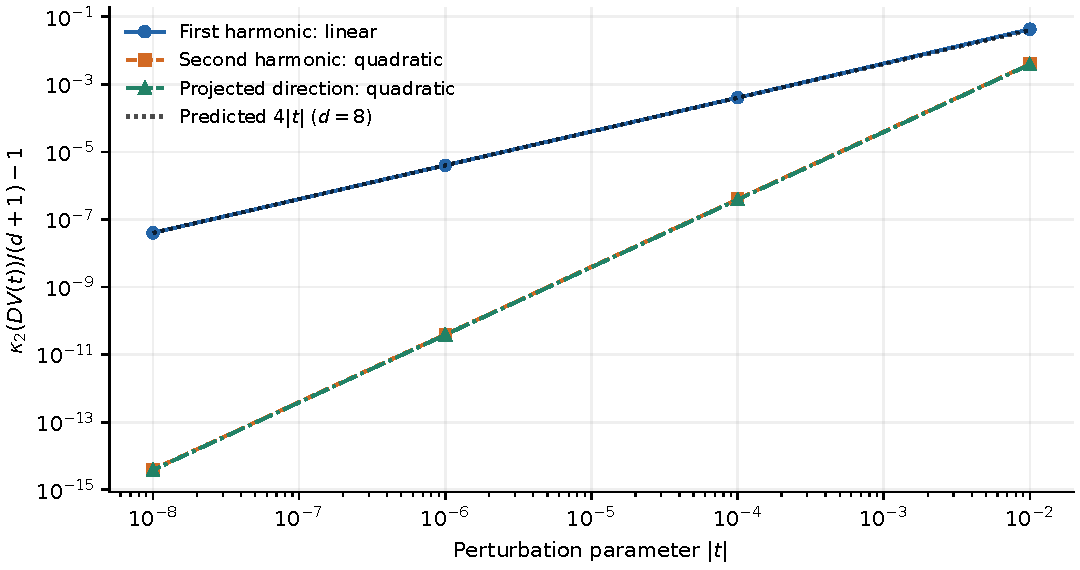
\includegraphics[width=.76\textwidth]{figures/directional_orders.pdf}
\caption{Local condition-number increments under the triangular weights with $d=8$.
First-order growth when the first harmonic is present; second-order growth for
non-rotational directions with vanishing first harmonic. The figure uses the 80-digit
computations.}\label{fig:directions}
\end{figure}


To assess the looseness of the upper bound of Proposition \ref{prop:near}, we take
$L=5,9,17$ with two families of positive weights: the triangular weights; and the
interior-minimum family $w_{\lfloor L/2\rfloor}=1$ with $w_n=2+n/L$ for the remaining
rows, whose largest and smallest weights are both attained once. For notational
simplicity we write its minimum row as $j=\lfloor L/2\rfloor$; the triangular weights
take $j=0$. The nodes are uniformly
\[
\beta_k(\varepsilon)=\exp\!\left(\frac{2\pi\ii}{L}(k+\varepsilon q_k)\right),
\qquad q_k=\frac{L(-1)^k-1}{L+1}.
\]
Here $\sum_kq_k=0$ and $\max_k|q_k|=1$, so $\varepsilon$ is the largest perturbation
fraction relative to the grid spacing. We take
\[
\varepsilon\in\{10^{-12},10^{-10},10^{-8},10^{-6},10^{-4},10^{-3},10^{-2},10^{-1}\},
\]
giving 48 cases, and additionally verify 6 equality configurations with $\varepsilon=0$.

Write $T_j$ and $H_{a,b}(\eta)$ for the left- and right-hand sides of
\eqref{eq:moment-bound}, and report $T_j/H_{a,b}(\eta)$ for the nonzero perturbations. All
cases satisfy the upper bound. For the interior-minimum weights the ratio lies between
about $0.250$ and $0.334$; for the triangular weights the ratio decreases markedly as
the perturbation shrinks, with a smallest measured value of about
$4.15\times10^{-12}$. The observed differences in bound tightness reflect the
distinct extreme-weight multiplicities of the two families.

\begin{figure}[htbp]\centering
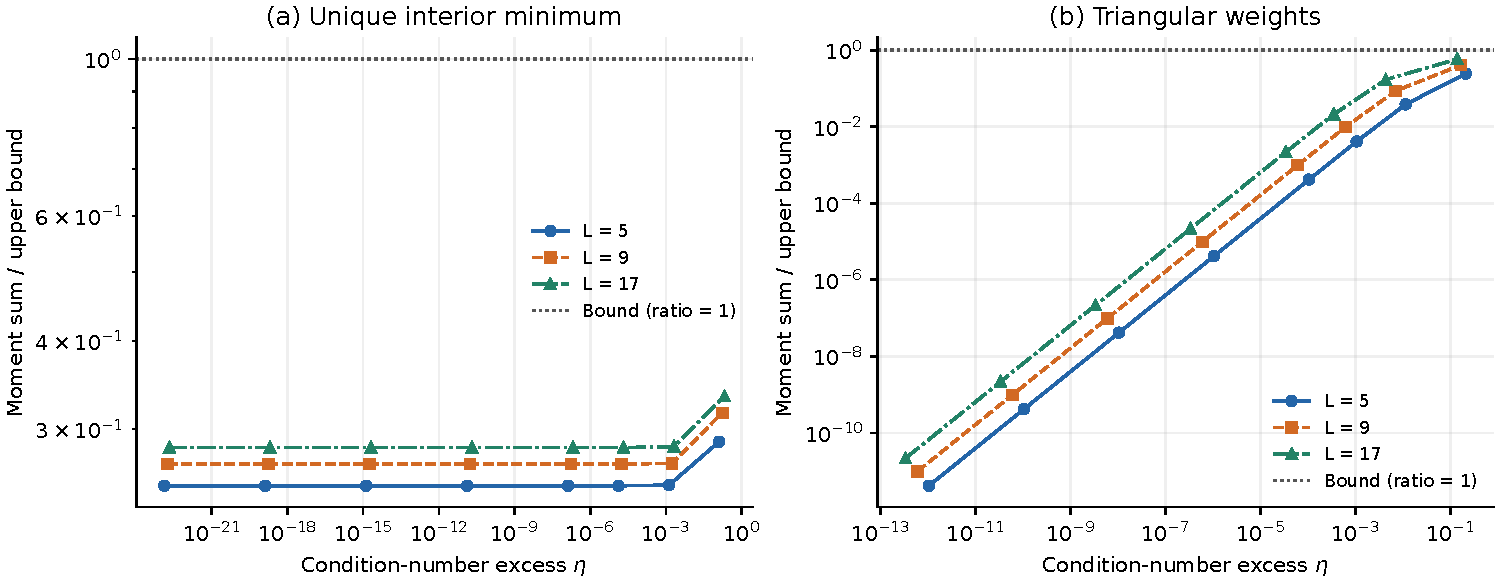
\includegraphics[width=.95\textwidth]{figures/moment_bound_ratio.pdf}
\caption{Ratio of the left-hand side of the near-optimal moment constraint to its upper
bound. Each curve corresponds to one fixed degree and a deterministic direction; the
dashed line marks ratio $1$. The two weight families illustrate different bound tightness
associated with their extreme-weight multiplicities.}\label{fig:moment-ratio}
\end{figure}


The difference is consistent with Theorem \ref{thm:directional}: in the interior-minimum
example both extremes are attained once and $\eta$ is second-order for non-rotational
directions, whereas for the triangular weights the present direction has a nonzero first
harmonic and $\eta$ is first-order. In both families $T_j$ is second-order, so the ratio
can retain a nonvanishing magnitude in the former and tends to zero in the latter.

\subsection{Computational accuracy and batch efficiency}

Define the weight forward error and the coefficient reconstruction residuals
\begin{equation}\label{eq:metrics}
E_\lambda=\frac{\norm{\widehat\lambda-\lambda_{\rm ref}}}{\norm{\lambda_{\rm ref}}},\qquad
R_{\rm dense}=\frac{\norm{\widehat M\widehat\lambda-A}}{\norm A},\qquad
R_{\rm fft}=\frac{\norm{D(L\operatorname{IFFT}(\widehat\lambda))-A}}{\norm A}.
\end{equation}
Here $(\operatorname{IFFT}z)_n=L^{-1}\sum_{k=0}^{L-1}z_k\e^{2\pi\ii nk/L}$,
and $\lambda_{\rm ref}$ is obtained by direct DFT summation at 80-digit precision, and
$\widehat M$ is constructed independently from floating-point nodes and successive
powers. FFT round trips may share numerical structure, so $R_{\rm fft}$ alone is not
used to certify the weight accuracy. We take $d=2,8,32,128$ and generate three instances
each of random complex coefficients, sparse coefficients with at most 4 nonzero entries,
and wide-scale coefficients whose moduli cover $10^{-8}$ to $10^8$, for 36 cases in
total.

\begin{table}[htbp]\centering\small
\caption{Largest errors over the nine cases of each degree, in e-notation.}\label{tab:accuracy}
\begin{tabular}{rrrrr}\toprule
$d$ & $L$ & $E_\lambda$ & $R_{\rm dense}$ & $R_{\rm fft}$\\\midrule
2 & 5 & 1.40e-16 & 6.31e-16 & 2.93e-16 \\
8 & 17 & 1.74e-16 & 1.53e-14 & 6.43e-16 \\
32 & 65 & 2.47e-16 & 4.85e-14 & 1.07e-15 \\
128 & 257 & 5.17e-16 & 2.61e-13 & 4.96e-15 \\
\\[-.8em]\bottomrule\end{tabular}
\end{table}

In Table \ref{tab:accuracy} the largest forward error of the ideal weights is about
$5.17\times10^{-16}$ and the largest dense-expansion residual about $2.61\times10^{-13}$;
the explicit node construction, power computation and summation add rounding, so the
three metrics need not coincide. A further 20 equality-case and 400 random cases verify
Proposition \ref{prop:perturb}; in the equality cases the normalized amplification
differs from $1$ by at most $1.52\times10^{-5}$, occurring at the smallest perturbations
and including the cancellation error of subtracting two floating-point solutions.

The batch experiment takes $d=8,32,128,512$ and $B=1,128$, using identical
complex128 inputs for the FFT, a precomputed dense operator, cached LU solves and
LU factorization followed by a solve at every call. Both LU methods use the same
SciPy routines and options. All methods are warmed up; their order is randomized
within each of 7 repetitions, with enough inner calls to reduce timer noise.
Figure \ref{fig:timing} reports median online times per batch, excluding input
generation and fixed-operator setup. The fresh-LU timing includes factorization;
the cached-LU timing excludes it. Preparation is reported in Table \ref{tab:setup}.
All solver outputs are also checked against the FFT weights and by dense residuals.

\begin{table}[htbp]\centering\small
\caption{Median preparation times in milliseconds. Stages are timed separately:
cached LU requires matrix construction and factorization; the dense transform
is constructed directly.}\label{tab:setup}
\begin{tabular}{rrrrr}\toprule
$d$ & Weights & Matrix $M$ & Dense operator $R$ & LU of $M$\\\midrule
% Generated values: repro/ela_revision/data/preparation_rows.tex
8 & 0.00396 & 0.0262 & 0.017 & 0.00819 \\
32 & 0.00342 & 0.315 & 0.129 & 0.0507 \\
128 & 0.00492 & 6.91 & 3.58 & 1.75 \\
512 & 0.00632 & 109 & 63.2 & 78.2 \\
\bottomrule\end{tabular}
\end{table}


\begin{figure}[htbp]\centering
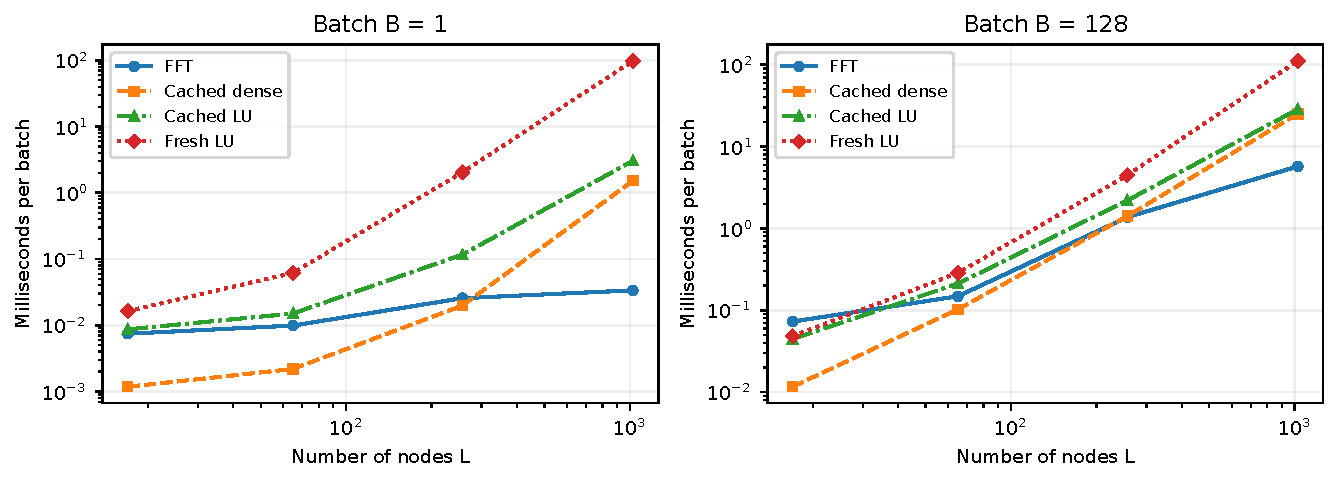
\includegraphics[width=.95\textwidth]{figures/batch_timings.pdf}
\caption{Median online timings per batch call; left panel $B=1$, right panel $B=128$.
Both cached methods reuse their preparation; fresh LU refactorizes at each call.}
\label{fig:timing}
\end{figure}

% BENCHMARK_RESULT_BEGIN
For $d=512$ and $B=128$, the FFT, cached dense transform, cached LU and fresh LU
take 5.73, 25.1, 28.6 and 111 ms per batch, respectively. 
At smaller sizes, the cached dense transform can be faster than the FFT;
the ordering also varies with batch size. Raw repetitions, setup times,
solver residuals and library records are supplied in \texttt{../code/ela\_revision};
the measurements describe this implementation and platform only.
% BENCHMARK_RESULT_END

\FloatBarrier
\section{Discussion and conclusion}\label{sec:conclusion}

For fixed nonzero monomial weights, the optimal unit-circle Vandermonde
configurations are exactly the rotated regular polygons. The local Fourier criterion
identifies which directions avoid linear growth, and the weighted moment constraint
ensures strictly quadratic growth in every non-rotational flat direction when the
weight moduli are unequal. Formula \eqref{eq:general-second} computes the coefficient
for every such direction, and \eqref{eq:coefficient-lower} gives positive lower bounds. For triangular weights, one Fourier coefficient decides
the order; the second harmonic also admits the explicit coefficient
\eqref{eq:second-harmonic}. By \eqref{eq:dimension-coefficient}, $C_d\sim2d^2/3$ in the
maximum-angular-displacement normalization of Remark \ref{rem:dimension};
removing linear growth therefore still leaves a dimension-dependent quadratic
sensitivity.

The geometric-square application supplies a fixed basis for binary forms. Its FFT
formula, Parseval identity and Kadec upper bound use existing tools; the experiments
check the local theory and distinguish ideal-weight accuracy from explicit-node
reconstruction errors. Cached LU and a precomputed dense transform provide reusable
baselines for the batch computation. Timing advantages remain dependent on matrix
size, batch size and implementation.

Questions left open include uniform control of higher-order remainders, node-matching
bounds from the moment constraint, and cancellation in real square factors.

\clearpage
\section*{Acknowledgements}
OpenAI ChatGPT (model label reported by the author: ChatGPT 6.1 sol) and
Codex assisted with Chinese-to-English translation, language editing, literature
discovery, proof-development suggestions for the local analysis in Section~3,
and preparation of the Python verification, plotting and benchmarking programs
in \texttt{../code}. Preliminary manuscript critiques from Gemini and Grok were
also considered; their model versions were not recorded in the available
revision materials. The numerical records were computed by the accompanying
programs. AI-generated critiques and finite computations do not constitute
independent peer review or mathematical proof. The human authors remain
responsible for verifying the arguments, citations, code and results before
submission and for the integrity and originality of the manuscript.
% The author supplied the ChatGPT model label; it is not independently certified.

\begin{thebibliography}{13}

\bibitem{aubel}
C. Aubel and H. B\"olcskei.
Vandermonde matrices with nodes in the
unit disk and the large sieve.
\emph{Appl. Comput. Harmon. Anal.}, 47:53--86, 2019.

\bibitem{bender}
M. R. Bender, J.-C. Faug\`ere, L. Perret, and E. Tsigaridas.
A nearly optimal algorithm to decompose binary forms.
\emph{J. Symbolic Comput.}, 105:71--96, 2021, \url{https://doi.org/10.1016/j.jsc.2020.06.002}.

\bibitem{berman}
L. Berman and A. Feuer.
On perfect conditioning of Vandermonde
matrices on the unit circle.
\emph{Electron. J. Linear Algebra}, 16:157--161, 2007.

\bibitem{bhatia}
R. Bhatia and C. Davis.
A better bound on the variance.
\emph{Amer. Math. Monthly}, 107:353--357, 2000.

\bibitem{chen}
X. Chen, R. S. Womersley, and J. J. Ye.
Minimizing the condition
number of a Gram matrix.
\emph{SIAM J. Optim.}, 21:127--148, 2011.

\bibitem{summation}
N. J. Higham.
The accuracy of floating point summation.
\emph{SIAM J. Sci. Comput.}, 14:783--799, 1993.

\bibitem{higham}
N. J. Higham.
\emph{Accuracy and Stability of Numerical Algorithms},
2nd ed., SIAM, Philadelphia, 2002.

\bibitem{kuian}
M. Kuian, L. Reichel, and S. V. Shiyanovskii.
Optimally conditioned
Vandermonde-like matrices.
\emph{SIAM J. Matrix Anal. Appl.}, 40:1399--1424, 2019.

\bibitem{pan}
V. Y. Pan.
How bad are Vandermonde matrices?
\emph{SIAM J. Matrix
Anal. Appl.}, 37:676--694, 2016, \url{https://doi.org/10.1137/15M1030170}.

\bibitem{reznick}
B. Reznick.
Some new canonical forms for polynomials.
\emph{Pacific J. Math.}, 266:185--220, 2013.

\bibitem{schatzman}
J. C. Schatzman.
Accuracy of the discrete Fourier transform and the
fast Fourier transform.
\emph{SIAM J. Sci. Comput.}, 17:1150--1166, 1996.

\bibitem{sharma}
R. Sharma and A. Thakur.
More inequalities for positive linear maps.
\emph{J. Math. Inequal.}, 7:1--9, 2013.

\bibitem{yu}
A. Yu and A. Townsend.
On the stability of unevenly spaced samples
for interpolation and quadrature. \emph{BIT Numer. Math.}, 63:Article 23, 2023.

\end{thebibliography}
\end{document}
